
\appendix

\begin{figure*}
    \centering
    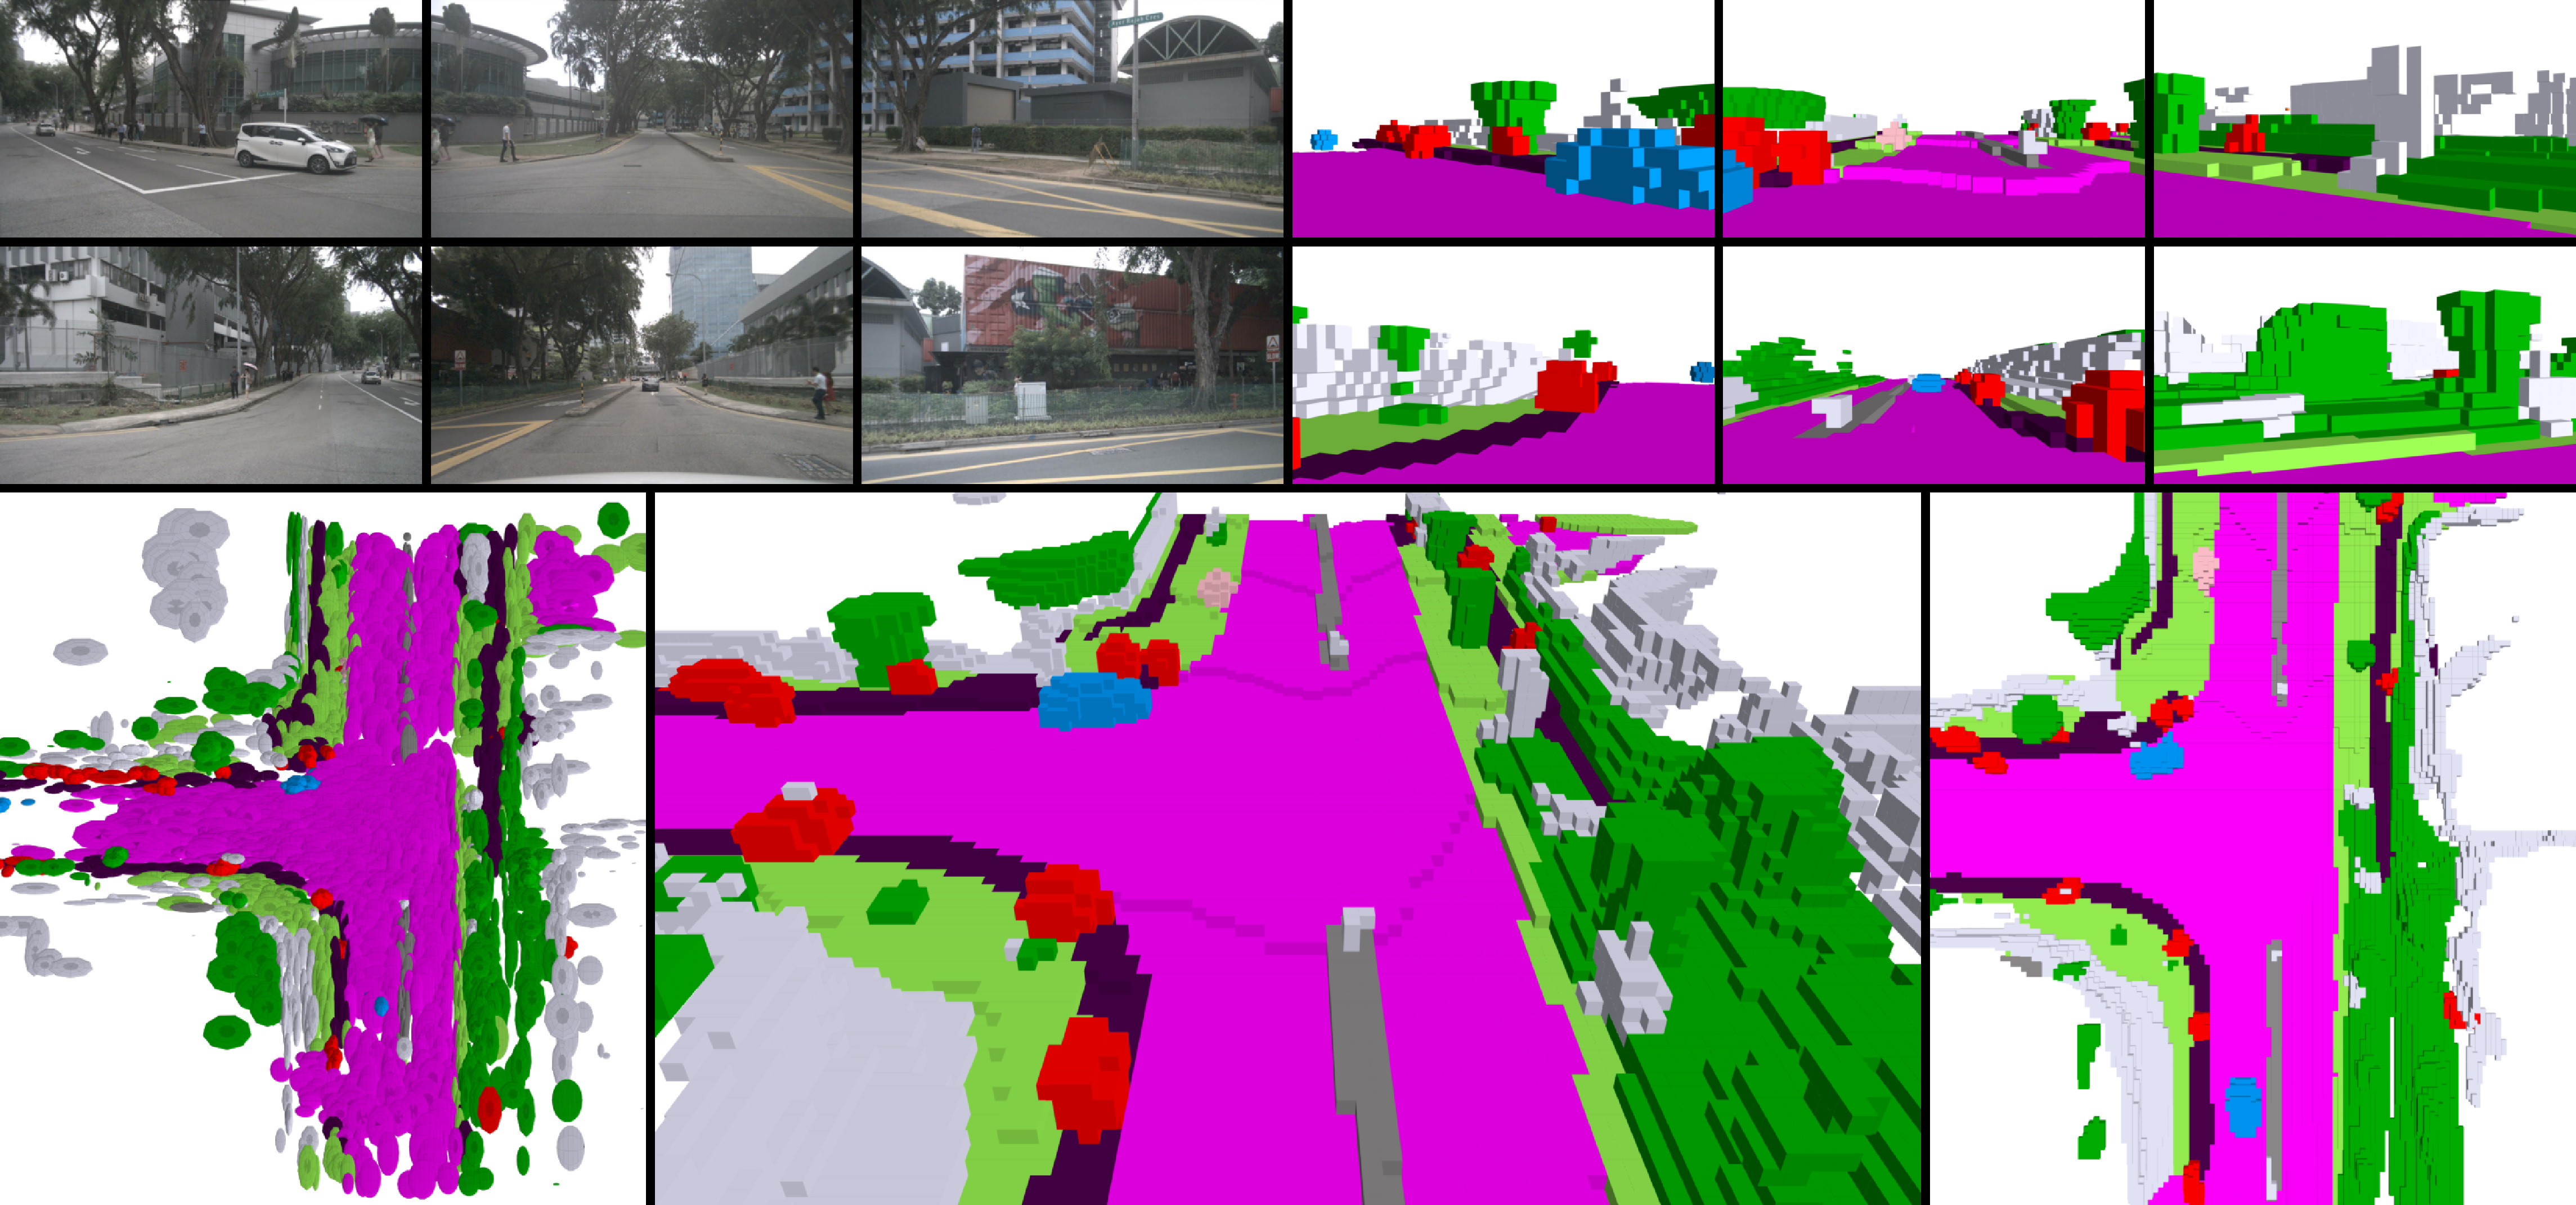
\includegraphics[width=\linewidth]{figures/supp_teaser.pdf}
    \vspace{-7mm}
    \captionof{figure}{
    \textbf{Visualizations of Gaussians, camera-view and overall occupancy on nuScenes.}
    We provide the input RGB images and their corresponding camera-view occupancy in the upper part.
    And we visualize the predicted 3D Gausians (left), the semantic occupancy in the global view (middle), and in the bird's eye view (right) in the lower part.
    }
\label{fig: supp teaser}
\end{figure*}%





\section{Video Demonstration}
\label{sec:video}
Figure~\ref{fig: supp teaser} shows a sampled frame of our video demonstration\footnote{\url{https://github.com/huang-yh/GaussianFormer}} for 3D semantic occupancy prediction on the nuScenes dataset~\cite{caesar2020nuscenes}.
We note that the camera-view occupancy visualizations align well with the input RGB images.
Moreover, each instance is sparsely described by only a few Gaussians with adaptive shapes, which demonstrates the efficiency and the object-centric nature of our model.


\section{Visualizations on KITTI-360}
\label{sec:vis kitti}
We provide visualization results of Gaussians and occupancy on the KITTI-360 dataset~\cite{Liao2022kitti360} in Figure~\ref{fig:supp kitti}.
We observe that our GaussianFormer-2 is able to predict both intricate geometry and semantics of the 3D scene.
Furthermore, the 3D Gaussians in our model are adaptive in their scales according to the specific objects they are describing, compared with isotropic spherical Gaussians with maximum scales in GaussianFormer~\cite{huang2024gaussian}.

\begin{figure*}[t]
\centering
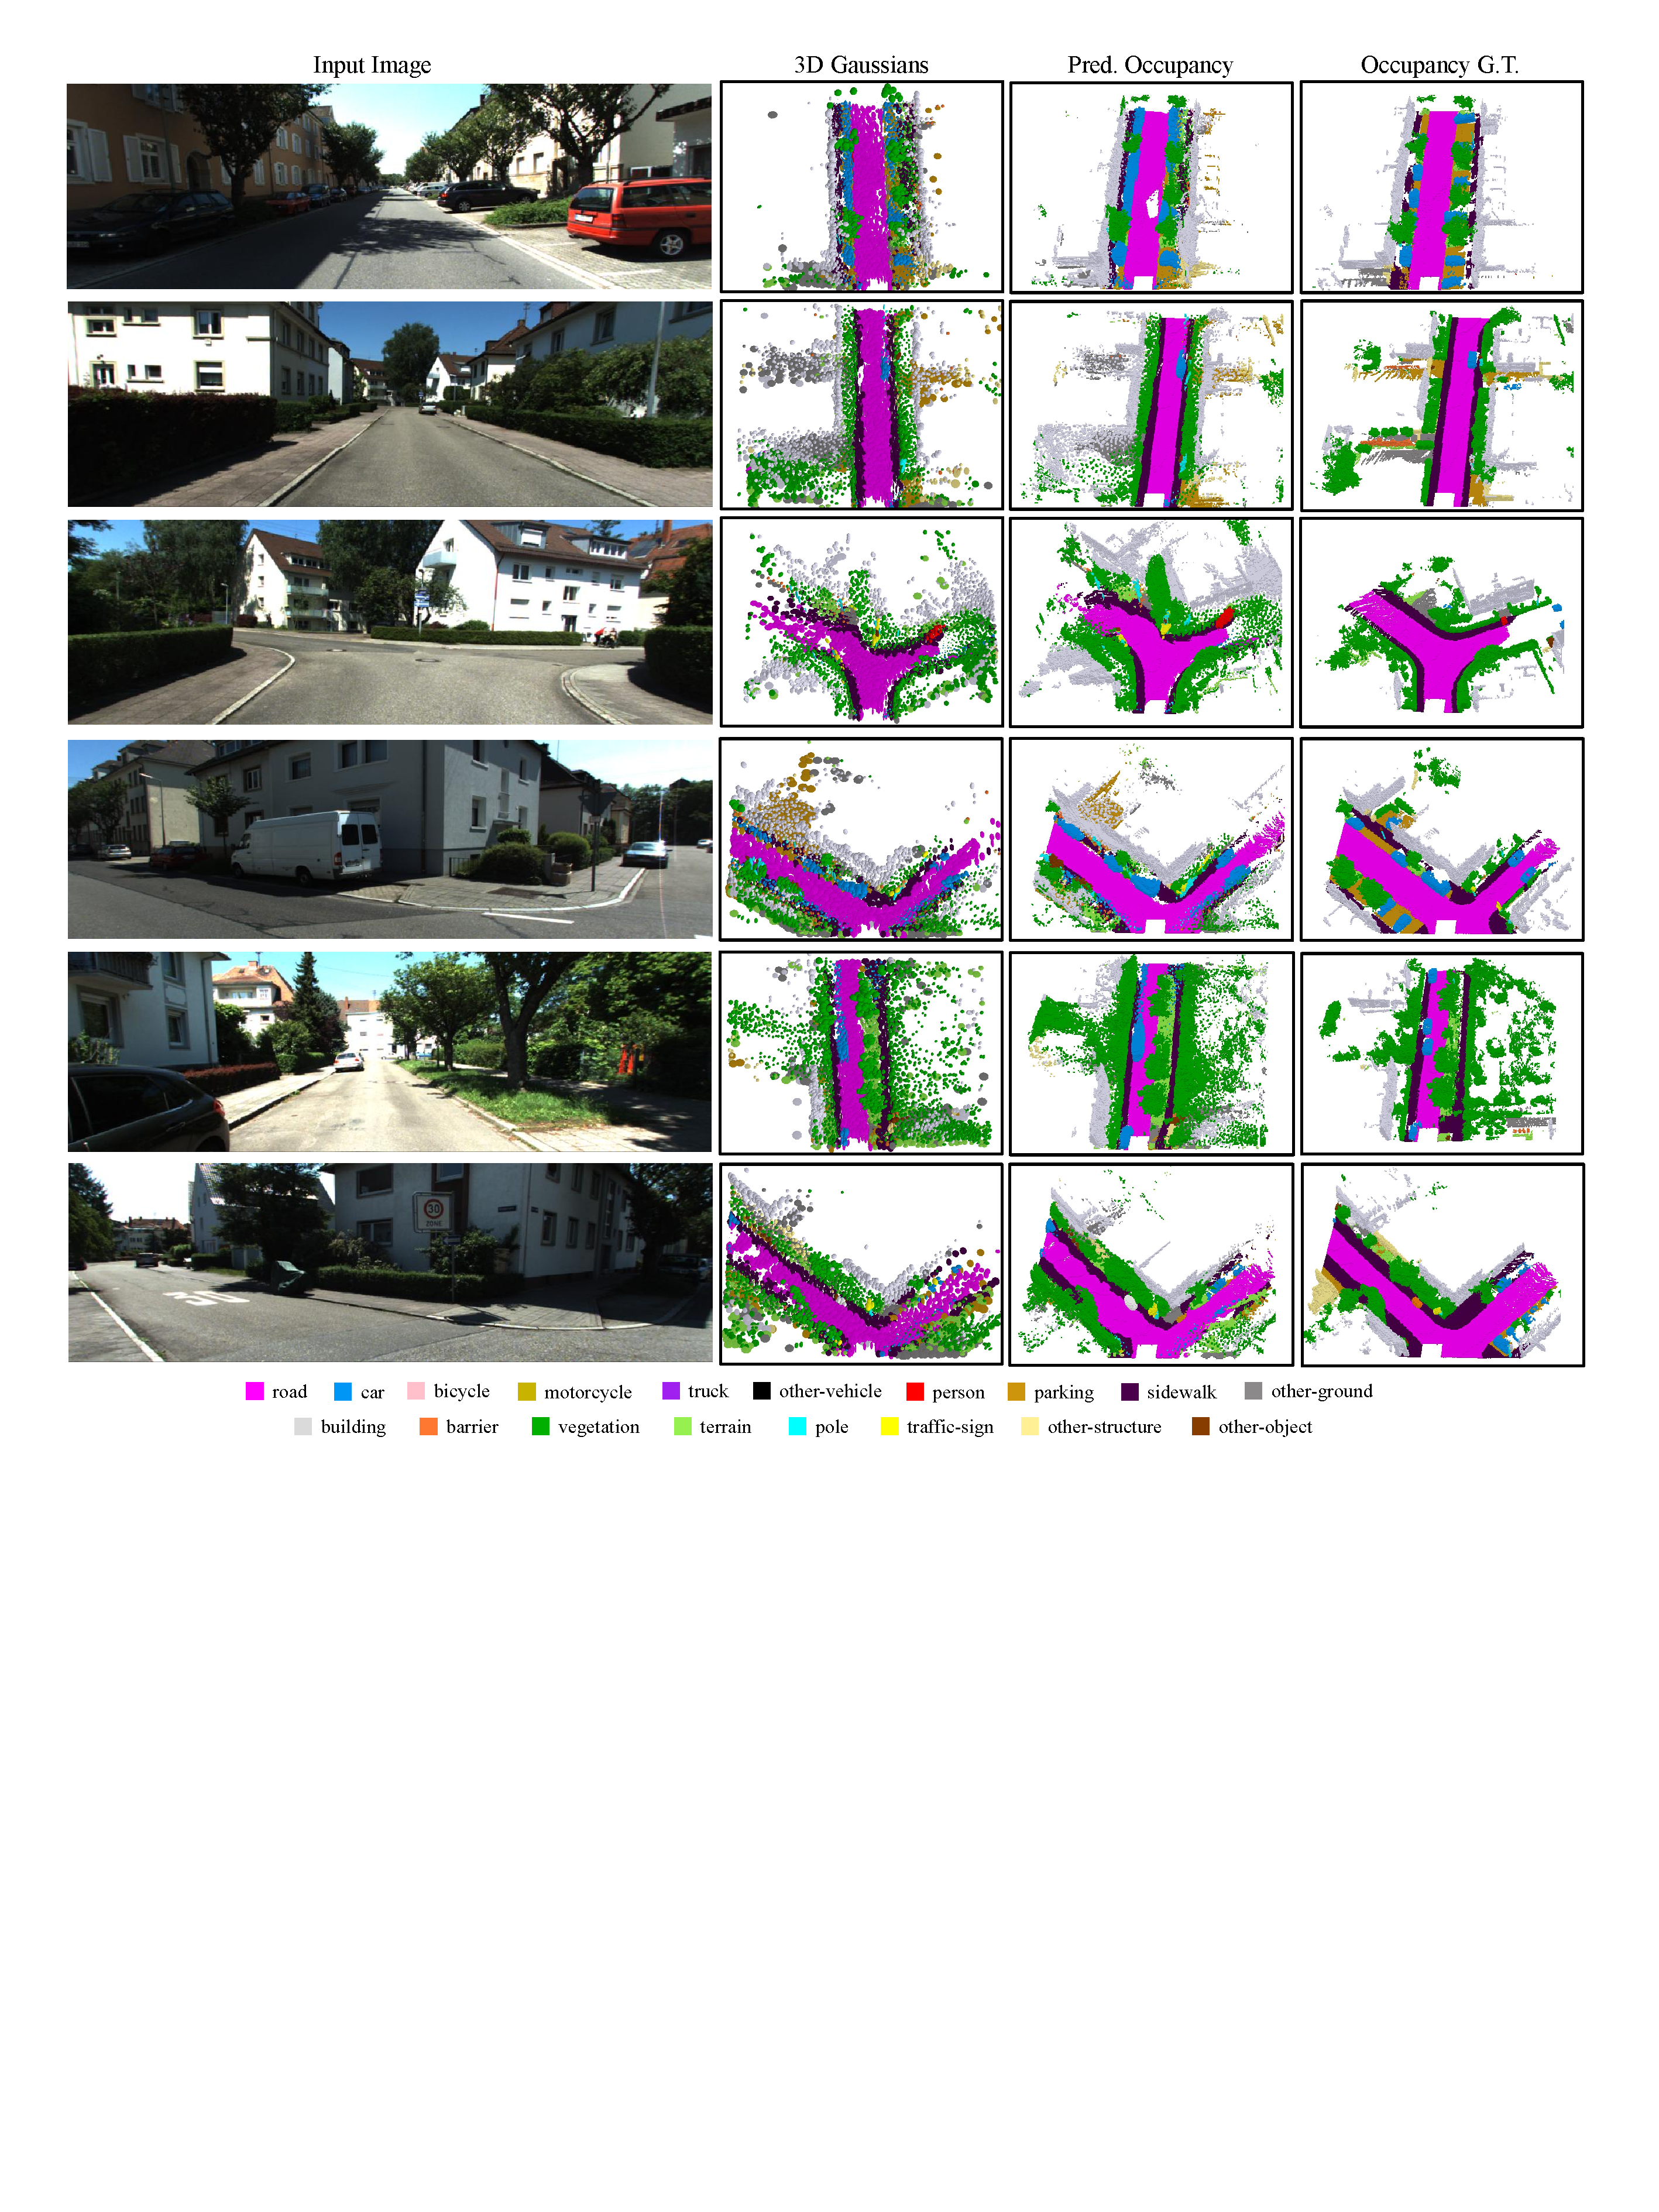
\includegraphics[width=0.95\linewidth]{figures/supp1.pdf}
\vspace{-2mm}
\caption{\textbf{Visualizations of Gaussians and occupancy on KITTI-360.}
Our method captures both the intricate geometry and semantics of the scene with shape-adaptive Gaussians.
}
\label{fig:supp kitti}
\vspace{-6mm}
\end{figure*}





\section{Metric Details}
\label{sec:efficiency metrics}

\textbf{Position.} 
Gaussians, even after full training, can still be found in unoccupied space due to the localized nature of the receptive field. 
These Gaussians fail to describe meaningful structures, rendering them ineffective and devoid of practical utility. 
A higher proportion of Gaussians in unoccupied space indicates suboptimal utilization. 
Hence, we define the \textit{percentage of Gaussians in correct positions (Perc.)} as:
\begin{equation}
    {\rm Perc.} = \frac{N_{\text{correct}}}{N_{\text{total}}} \cdot 100\%,
    \label{eq: Perc.}
\end{equation}
where $N_{\text{correct}}$, and $N_{\text{total}}$ denote the number of Gaussians of which means are in occupied space, and the total number of Gaussians, respectively. 
A higher percentage indicates a better alignment of the Gaussians with occupied or meaningful area in the space, thus reflecting a more efficient use of the model's capacity.

The above measurement provides a hard evaluation, where Gaussians are either classified as being in correct or incorrect positions without considering their proximity to the nearest occupied area. 
This binary approach does not capture how close Gaussians in unoccupied regions are to meaningful positions. 
To address this limitation, we define a complementary soft measurement as the average distance of each Gaussian to its nearest occupied voxel center, denoted as \textit{Dist.} (in meters), computed as follows:
\begin{equation}
    {\rm Dist.} = \frac{1}{P} \sum_{i=1}^{P} \underset{\mathbf{v} \in \mathcal{V}}{\rm min} ||\mathbf{m}_i - \mathbf{v}||_1,
    \label{eq: Dist.}
\end{equation}
where $\mathbf{m}_i$, $\mathcal{V}$, $\mathbf{v}$, and $||\mathbf{m}_i - \mathbf{v}||_1$ denote the mean of the i-th Gaussian, the set of occupied voxel centers, the center of one voxel in this set, and L1 distance between the mean of the Gaussian and the voxel center, respectively.
Note that this distance is calculated with respect to the voxel center, and thus Gaussians positioned within the correct occupied area may also have a non-zero distance.


\textbf{Overlap.} 
The \textit{overall overlapping ratio of Gaussians (Overall.)} provides a global perspective on the redundancy in the Gaussian representation. 
Each Gaussian is modeled as an ellipsoid, where the semi-axis lengths are derived from the Mahalanobis distance at a chi-squared value of 6.251, corresponding to the 90\% confidence level of a Gaussian distribution in three degrees of freedom (DoFs).
The \textit{Overall.} is then calculated as the ratio of the summed 90\% confidence volumes $V_{i,90\%}$ of all Gaussians to the total coverage volume of all Gaussians $V_{\text{coverage}}$ in the scene:
\begin{equation}
    {\rm Overall.} = \frac{\sum_{i=1}^{P} V_{i,90\%}}{V_{\text{coverage}}}, 
    \label{eq: Overall.}
\end{equation}
where $V_{\text{coverage}}$ represents the volume of all Gaussians combined as a unified shape. To estimate $V_{\text{coverage}}$, we employ the \textit{Monte Carlo method} where a large number of points are randomly sampled within the bounding box of the scene. For each sampled point, we check whether it lies within the 90\% confidence ellipsoid of any Gaussian. The volume is then approximated as:
\begin{equation}
    V_{\text{coverage}} = V_{\text{scene}} \cdot \frac{N_{\text{in}}}{N_{\text{total}}},
    \label{eq: Monte}
\end{equation}where $N_{\text{in}}$, and $N_{\text{total}}$ are the number of sampled points that fall within the 90\% confidence ellipsoid of at least one Gaussian, and the total number of sampled points, respectively. This approach ensures an accurate estimation of the unified volume, efficiently handling the overlapping regions of the Gaussians by not double-counting them.

We next detail the derivation of the ellipsoid volume corresponding to the 90\% confidence region of a 3D Gaussian distribution. 
Considering a multivariate Gaussian distribution in 3D defined as:

\vspace{-4mm}
\begin{small}
\begin{equation}
    \mathbf{g}(\mathbf{x}) = \frac{1}{(2 \pi)^{3/2}|\mathbf{\Sigma}|^{1/2}}{\rm{exp}}\big(-\frac{1}{2}(\mathbf{x}-\mathbf{m})^{\rm T} \mathbf{\Sigma}^{-1} (\mathbf{x}-\mathbf{m})\big),
    \label{eq: gaussian_dist}
\end{equation}
\end{small}where $\mathbf{x}$, $\mathbf{\Sigma}$, and $|\mathbf{\Sigma}|$ are the mean vector, 3x3 covariance matrix, and the determinant of the covariance matrix, respectively.
The \textit{Mahalanobis distance} $d$ of point $\mathbf{x}$ from the mean $\mathbf{m}$ is defined as:
\begin{equation}
    d^2(\mathbf{x},\mathbf{m}) = (\mathbf{x}-\mathbf{m})^{\rm T} \mathbf{\Sigma}^{-1} (\mathbf{x}-\mathbf{m}).
    \label{eq: maha_dist}
\end{equation}
The 90\% confidence region of the Gaussian distribution corresponds to the set of points for which the Mahalanobis distance satisfies:
\begin{equation}
    d^2 \le \chi_{3,0.9}^2 \approx 6.251,
    \label{eq: chi2}
\end{equation}
where $\chi_{3,0.9}^2$ is the chi-square critical value for three degrees of freedom at the 90\% confidence level.
For a Gaussian distribution, the semi-axis lengths are determined by the square root of the eigenvalues of $\mathbf{\Sigma}$, scaled by $\chi_{3,0.9}^2$.
Thus, the volume of the ellipsoid from 90\% of the 3D Gaussian distribution is:
\begin{equation}
    V_{90\%} = \frac{4}{3}\pi (6.251)^{3/2} |\mathbf{\Sigma}|^{1/2}.
    \label{eq: V_2}
\end{equation}
A higher value of \textit{Overall.} indicates greater overlapping volumes among the Gaussians, signifying redundancy in Gaussian representation. 
This metric provides insights into the utilization of Gaussians to represent the scene.

The \textit{individual overlapping ratio of Gaussians (Indiv.)} offers a fine-grained analysis of the overlap between Gaussians in a scene. 
This measurement quantifies the degree to which each Gaussian overlaps with all other Gaussians, averaged across all Gaussians in the scene. 
The value of this metric indicates approximately how many times the volume of a single Gaussian is fully overlapped with other Gaussians on average.
To compute this, we use the Bhattacharyya coefficient~\cite{bhattacharyya1943bhatcoef}, which measures the similarity between two Gaussian distributions. 
The \textit{individual overlapping ratio} is defined as:
\begin{equation}
   {\rm Indiv.} = \frac{1}{P}\sum_{i=1}^{P}\left(\sum_{j\ne i}{\rm BC}_{i,j}\right),
    \label{eq: indiv}
\end{equation}
where ${\rm BC}_{i,j}$ is the Bhattacharyya coefficient between the i-th and j-th Gaussians, given by:
\begin{equation}
   {\rm BC}_{i,j} = \frac{\sqrt[4]{|\mathbf{\Sigma}_i||\mathbf{\Sigma}_j|}}{\sqrt{|\mathbf{\Sigma}_{ij}|}}e^{-\frac{1}{8}(\mathbf{m}_i-\mathbf{m}_j)^{\rm T}\mathbf{\Sigma}_{ij}^{-1}(\mathbf{m}_i-\mathbf{m}_j)},
   \label{eq: Batta}
\end{equation}
where $\mathbf{\Sigma}_{ij}=\frac{1}{2}(\mathbf{\Sigma}_i+\mathbf{\Sigma}_j)$ is the average covariance matrix.
A higher value of \textit{Indiv.} indicates more redundancy, as Gaussians are heavily overlapping with each other.
